\chapter{Introducción}
\label{cap:intro}
%\chapterquote{Hablaban siempre de dinero y planeaban asaltar un banco}{Domingo Cavallo, 2001}


\subsection*{Fenómeno de Convección}

Desde un punto de vista general, el fenómeno de convección hace referencia al transporte de calor debido al movimiento de un fluido. En ingeniería es común utilizar el término convección para describir la transferencia de calor desde una superficie hacia un fluido en movimiento cuando ambos están a diferentes temperaturas \cite{cengelheat,incropera}. 

La transferencia de calor por convección puede clasificarse según la naturaleza del flujo. Se habla de convección forzada cuando el flujo es provocado por actores externos \textcolor{black}{como puede ser la acción de una bomba que impulsa el flujo}; en cambio, en la convección natural, el flujo es inducido por fuerzas boyantes o de flotación, las cuales, en general, surgen debido a diferencias de densidad producidas por variaciones de temperatura en el propio fluido (Figura \ref{fig:natural_forzada}).



\begin{figure}[H]
 \centering
    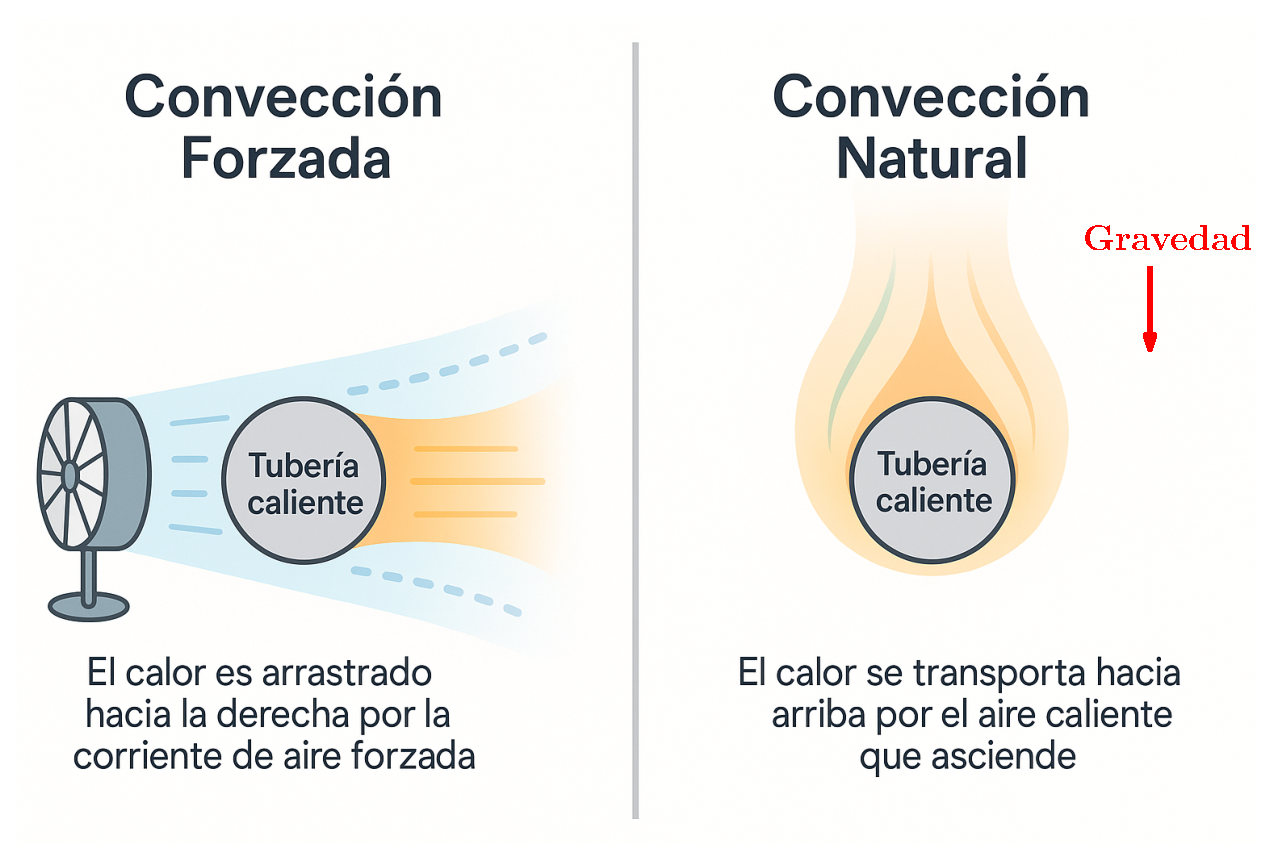
\includegraphics[width=0.6\textwidth]{figures/cap1/natural_forzada.eps}
    \label{fig:natural_forzada} 
 \caption{Comparación esquemática de la transferencia de calor alrededor de una tubería caliente: (izquierda) convección forzada; (derecha) convección natural.} 
 \label{fig:natural_forzada}
\end{figure}

Los primeros estudios sobre la transferencia de calor por convección trataron las ramas de la convección forzada y la convección natural de forma separada, sin considerar \linebreak la posible interacción entre ambas. Por un lado, los experimentos de Henri Bénard (1901) marcaron un hito en la comprensión de la convección natural \cite{benard1901}. Bénard mostró que una lámina delgada de líquido con superficie libre, sometida a un gradiente térmico, desarrolla espontáneamente una circulación en celdas de simetría hexagonal (las ``celdas de Bénard'') y, mediante métodos ópticos, registró y midió su geometría y escala. Más tarde, Lord Rayleigh (1916) desarrolló la base teórica de la inestabilidad térmica en capas fluidas \cite{rayleigh1916}. En paralelo, en el ámbito de la convección forzada, trabajos como el de Dittus y Boelter (1930) establecieron correlaciones empíricas para la transferencia de calor en tubos \cite{dittus1930}. No fue sino hasta mediados del siglo XX que comenzó a reconocerse que ambos mecanismos pueden coexistir en muchas configuraciones de interés práctico. Así surgió el concepto de convección mixta, donde la convección forzada y la natural actúan simultáneamente como casos extremos de un fenómeno más general \cite{metais1964}. 

\subsection*{Transición Laminar-Turbulenta y efectos de la convección}

Cuando un fluido se desplaza a través de un conducto o sobre una superficie, su movimiento puede clasificarse en dos tipos de régimen: laminar o turbulento \cite{white}. En el régimen laminar, el flujo es ordenado y las partículas del fluido se mueven en capas paralelas sin mezclarse entre sí. En cambio, en el régimen turbulento, el flujo es caótico, con remolinos, tiende a mezclarse, y presenta fluctuaciones en los campos de velocidad y presión \cite{kundu}. \textcolor{black}{Asimismo, si un flujo se encuentra en un estado intermedio entre laminar y turbulento, y además no se desarrolla (es \linebreak decir, se mantiene de esa forma en el tiempo y en el espacio), se dice que el flujo está en régimen de transición.} Este aspecto puede presentarse, por ejemplo, en el diseño de \linebreak intercambiadores de calor: el punto de operación del flujo dentro de los tubos o conductos podría situarse en régimen de transición, en cuyo caso las magnitudes relevantes (como coeficientes de fricción y de transferencia de calor) experimentan variaciones significativas \cite{ghajar2019heat}. 


\textcolor{black}{Por otro lado, el régimen de transición no debe confundirse con la transición laminar-turbulenta del sistema, donde el flujo evoluciona de un régimen laminar a un régimen turbulento completamente desarrollado}\footnote{Esto significa que los perfiles de las magnitudes de interés (como la velocidad) no varían a lo largo de la dirección del flujo. En régimen turbulento, esto se entiende en el sentido estadístico: son los promedios de dichas magnitudes los que no cambian.}. \textcolor{black}{Esta transición puede ocurrir en el tiempo (transición laminar-turbulenta temporal) o en el espacio (transición laminar-turbulenta espacial)} \cite{schlatter2005}:

\begin{itemize}

\item \textcolor{black}{En una \textbf{transición temporal}, el flujo cambia con el tiempo en un dominio fijo. Es decir, las condiciones iniciales son impuestas y se observa cómo el flujo evoluciona desde un estado laminar hasta uno turbulento con el transcurso del tiempo.}

\item \textcolor{black}{En una \textbf{transición espacial}, en cambio, el flujo es estacionario en el tiempo, pero las propiedades varían a lo largo de la dirección del flujo: el fluido entra laminar y se vuelve turbulento conforme avanza por el dominio.
}
\end{itemize}
Este fenómeno es de gran importancia para la ingeniería y la física aplicada ya que está presente en diferentes dispositivos termohidráulicos. En este sentido, el cambio de un régimen a otro puede tener un impacto significativo en los parámetros característicos del flujo. En general, el coeficiente de fricción (factor de Darcy) o el coeficiente de convección (número de Nusselt) se incrementan notablemente cuando se produce la transición \cite{incropera,white}. Por ello, caracterizar la transición entre los regímenes laminar y turbulento es fundamental para controlar el fenómeno y anticipar su comportamiento.

Esta transición puede ocurrir en el tiempo (transición laminar-turbulenta temporal), cuando un flujo inicialmente laminar se vuelve turbulento conforme evoluciona en el tiempo bajo condiciones iniciales fijas, o en el espacio (transición laminar-turbulenta espacial), cuando el flujo se mantiene estacionario pero pasa de laminar a turbulento a lo largo de la dirección del flujo.


La investigación teórica sobre la transición ha tenido un desarrollo histórico notable que se remonta al siglo XIX, con el célebre experimento de Osborne Reynolds \cite{reynolds1883}, que marcó el inicio del estudio sistemático del fenómeno. A comienzos del siglo XX, Orr \cite{orr1907} y Sommerfeld \cite{sommerfeld1908} formalizaron las bases de la estabilidad hidrodinámica al desarrollar las ecuaciones linealizadas que llevan sus nombres, conocidas como ecuaciones de Orr-Sommerfeld. Estas describen la evolución de perturbaciones en un flujo y son fundamentales para comprender los mecanismos de transición. Un avance crucial se produjo con los trabajos de Tollmien \cite{tollmien1930} y Schlichting \cite{schlichting1933}, quienes describieron de forma teórica el estado lineal de la transición; esta teoría fue confirmada experimentalmente en el estudio de la capa límite sobre una placa plana realizado por Schubauer y Skramstad \cite{schubauer1947laminar}. Finalmente, la incorporación de la teoría de inestabilidad secundaria por Herbert \cite{herbert1983secondary} permitió extender el análisis al caso tridimensional, ofreciendo así una comprensión más completa del fenómeno. 

Cabe destacar que los trabajos mencionados en el párrafo anterior tienen en consideración únicamente flujos isotérmicos. En el contexto de estudios que involucran la convección natural y/o la convección forzada, los trabajos experimentales de Scheele \textit{et al.}  \cite{scheele1960effect, scheele1962effect} mostraron que el flujo en una tubería vertical calentada puede experimentar una transición a números de Reynolds (basados en el radio de la tubería) inferiores a 1800. Para estos valores, Scheele y \linebreak  Hanratty \cite{scheele1962effect} hallaron que, en condiciones de calentamiento con flujo ascendente, la inestabilidad aparece cuando los perfiles de velocidad \linebreak  desarrollan puntos de inflexión. La transición hacia un régimen no estacionario procede mediante el crecimiento paulatino de pequeñas perturbaciones; por ello, si la tubería no es lo suficientemente larga, no es posible observar la transición del flujo. En paralelo, en el plano analítico, Tao \cite{tao1960} estudió el flujo laminar totalmente desarrollado con convección mixta en un canal vertical, y explicitó las soluciones a partir de las cuales pueden desarrollarse las ecuaciones de Orr-Sommerfeld.

Décadas más tarde, Gebhart \textit{et al.} \cite{gebhart1989buoyancy} realizaron una discusión exhaustiva sobre los flujos inducidos por flotación y destacaron que los mecanismos de transición en convección mixta difieren de los correspondientes al flujo isotérmico. En esa línea, los análisis de estabilidad lineal de Chen y Chung para el flujo en un canal vertical con distintas condiciones de calentamiento en las paredes \cite{chen1996linear,chen1998stability} mostraron que la transferencia de calor desestabiliza el sistema. En consecuencia, el flujo calentado y plenamente desarrollado resulta inestable y la transición ocurre a números de Reynolds relativamente bajos.

Desde el punto de vista numérico, mediante simulación directa (DNS), Chen y Chung \cite{chen2002direct} estudiaron la transición para un flujo levemente forzado con bajo número de Reynolds en un canal vertical calentado. Asimismo, analizaron el fenómeno de transición laminar-turbulenta en convección mixta asistida por flotación \cite{chen2003direct}.

A partir de todo lo mencionado hasta aquí, se puede inferir que la evolución de un flujo, en el tiempo y en el espacio, depende de perturbaciones externas, condiciones de borde y de la respuesta del sistema, fijada por sus propiedades físicas y el régimen de flujo. En ese sentido, existen diversos factores que pueden desencadenar la transición del flujo, como por ejemplo la rugosidad o el espesor de las paredes, entre muchos otros. En este trabajo se emplea uno de los posibles mecanismos de inestabilización: las perturbaciones que resultan de la teoría de estabilidad lineal \cite{schmid}. 

La idea consiste en producir estados o condiciones iniciales capaces de desencadenar una transición con la intención de analizar cómo la misma impacta en la transferencia de calor. Esta teoría ofrece un marco para predecir cuándo un flujo laminar se volverá inestable mediante el estudio de la evolución de pequeñas perturbaciones: si estas crecen en el espacio o en el tiempo, el flujo pierde su estabilidad y eventualmente transiciona hacia un régimen turbulento.


\section{Motivación}

En la mayoría de aplicaciones en ingeniería, los flujos involucrados son no isotérmicos \cite{chen2003direct}. En ese sentido, la convección mixta en canales y conductos verticales se encuentra presente en muchos sistemas de interés; entre ellos los intercambiadores de calor, los cuales se encuentran integrados a su vez en sistemas más complejos (como centrales termoeléctricas) y son ampliamente utilizados en procesos industriales. Mejorar la eficiencia de estos equipos es vital ya que impacta directamente en el consumo energético y en los costos de producción.

Por otro lado, este tipo de sistemas pueden presentar cambios de régimen (laminar-turbulento) en su evolución \cite{schlatter2005}. Desde el punto de vista ingenieril, las características del cambio de régimen son de gran relevancia ya que, como se ha mencionado anteriormente, parámetros de interés como el número de Nusselt pueden variar considerablemente cuando se pasa de un régimen a otro. Por lo cual, el estudio de la transferencia de calor en canales verticales con flujos en transición laminar-turbulenta y en convección mixta, resulta importante para predecir cómo la fuerza boyante y el flujo forzado modifican el intercambio térmico (Nu) y las pérdidas por fricción ($f$) a lo largo de la transición. A partir de ello, es posible establecer criterios de diseño y una operación más eficiente y segura.




\section{Objetivos}

El objetivo del presente trabajo es el estudio de la transferencia de calor en \linebreak régimen de transición laminar-turbulenta en convección mixta. Para ello se emplea la herramienta numérica Xcompact3D. Se obtienen resultados numéricos para distintos números de Reynolds (Re), números de Prandtl (Pr) y números de Richardson (Ri). A partir de dichos resultados se calculan magnitudes de interés como por ejemplo el número de Nusselt y/o el factor de fricción de Darcy. Luego, por un lado, se analiza cómo estas cantidades se modifican  con la variación de Re, Pr y Ri (estado estadísticamente estacionario), y por el otro, cómo se modifican en el tiempo para los casos de transición. Parte de las tareas secundarias para la realización del trabajo incluyeron:

\begin{itemize}

	\item Entrenamiento y manejo en el uso de la herramienta numérica Xcompact3D \linebreak \cite{bartholomew2020xcompact3d}.
	
	\item Validación de la herramienta numérica y simulación de flujos turbulentos.

	\item Utilización y validación de la herramienta numérica OSMC \cite{szuban2023} para inestabilizar flujos a partir de soluciones laminares mediante perturbaciones \linebreak generadas por la teoría de estabilidad lineal.

\end{itemize}

\section{Organización del trabajo}

El trabajo se organiza en siete capítulos. En el Capítulo \ref{cap:modelo} se presenta un breve marco teórico, que incluye las ecuaciones de gobierno, las condiciones de borde y los conceptos necesarios para comprender el problema, así como la teoría de estabilidad lineal y las soluciones laminares utilizadas en la construcción de perturbaciones. El Capítulo \ref{cap:numerico} describe los métodos numéricos en los que se basan las herramientas de simulación empleadas. En el Capítulo \ref{cap:validacion} se lleva a cabo la validación de las herramientas numéricas utilizadas, Xcompact3D y OSMC.

El Capítulo \ref{cap:desarrollado} presenta los resultados principales para flujo turbulento desarrollado con convección mixta. Incluye perfiles de velocidad y temperatura y la comparación de Nu y del factor de Darcy frente a correlaciones y datos de referencia. En el Capítulo \ref{cap:transicion} se realiza una breve exploración de casos para determinar qué condiciones iniciales, generadas con OSMC, producen la inestabilización del flujo. A continuación, se analiza la evolución temporal de magnitudes relevantes para estudiar la transición del régimen laminar al turbulento.

Finalmente, en el Capítulo \ref{cap:conclusiones} se resumen los aportes del trabajo y se presentan las conclusiones más relevantes.